%% ─────────────────────────────────────────────────────────────────────────────
%% System Architecture Overview
%% Two figures: (1) five-stage annotation pipeline, (2) sensor configuration
%% ─────────────────────────────────────────────────────────────────────────────

\subsection{System Architecture Overview}
\label{ssec:arch_overview}

Figure~\ref{fig:pipeline} illustrates the five-stage \lucid{} data pipeline from
fleet deployment through public benchmark release. Figure~\ref{fig:sensor_config}
provides a top-down schematic of the sensor configuration on each collection vehicle,
showing camera fields of view, LiDAR coverage rings, and radar beam directions.

%% ── Figure 1: Five-stage Annotation Pipeline ─────────────────────────────────
\begin{figure*}[htbp]
\centering
\resizebox{\linewidth}{!}{%
\begin{tikzpicture}[
  font=\small,
  mbox/.style={%
    draw, rounded corners=5pt,
    minimum width=2.60cm, minimum height=5.20cm,
    text width=2.45cm, align=center,
    inner sep=5pt, line width=0.9pt},
  farrow/.style={->, >=Stealth, line width=2.2pt},
  st1/.style={mbox, fill=blue!9!white,   draw=blue!55!black},
  st2/.style={mbox, fill=teal!9!white,   draw=teal!55!black},
  st3/.style={mbox, fill=orange!9!white, draw=orange!55!black},
  st4/.style={mbox, fill=violet!9!white, draw=violet!55!black},
  st5/.style={mbox, fill=green!9!white,  draw=green!55!black},
]

%% ── Stage nodes ─────────────────────────────────────────────────────────────
\node[st1] (S1) at (0,0) {%
  \textbf{\textcolor{blue!75!black}{Stage 1}}\\[3pt]%
  \textbf{Data Collection}\\[6pt]%
  \footnotesize%
  3 vehicle fleets\\%
  6 cities / 3 continents\\[4pt]%
  8 cameras\\%
  5 LiDARs\\%
  5 radars\\%
  GPS/IMU, HD maps\\[4pt]%
  \textit{107 hours total}%
};

\node[st2] (S2) at (3.3,0) {%
  \textbf{\textcolor{teal!75!black}{Stage 2}}\\[3pt]%
  \textbf{Preprocessing}\\[6pt]%
  \footnotesize%
  Sensor alignment\\%
  PTP sync\\%
  Segmentation\\%
  Quality filter\\%
  Anonymisation\\%
  3D object tracking\\[4pt]%
  \textit{12{,}847 scenarios}%
};

\node[st3] (S3) at (6.6,0) {%
  \textbf{\textcolor{orange!75!black}{Stage 3}}\\[3pt]%
  \textbf{Annotation}\\[6pt]%
  \footnotesize%
  Scene descriptions\\%
  Agent labels\\%
  Causal chain QA\\%
  Counterfactual QA\\%
  Risk assessment\\%
  Planning instruct.\\[4pt]%
  \textit{234 annotators}%
};

\node[st4] (S4) at (9.9,0) {%
  \textbf{\textcolor{violet!75!black}{Stage 4}}\\[3pt]%
  \textbf{Quality Control}\\[6pt]%
  \footnotesize%
  Cross-review pass\\%
  Expert validation\\%
  IAA computation\\%
  BERTScore filter\\%
  Plausibility check\\[4pt]%
  $\kappa{>}0.80$\\%
  \textit{45K person-hours}%
};

\node[st5] (S5) at (13.2,0) {%
  \textbf{\textcolor{green!75!black}{Stage 5}}\\[3pt]%
  \textbf{Benchmark Release}\\[6pt]%
  \footnotesize%
  70/15/15\% split\\%
  4 benchmark tasks:\\%
  CSU, CFR, IFN, RAP\\[3pt]%
  Eval.\ server\\%
  Baseline code\\%
  Model checkpoints\\[4pt]%
  \textit{CC BY-NC 4.0}%
};

%% ── Forward arrows ──────────────────────────────────────────────────────────
\draw[farrow, blue!55!black]   (S1.east) -- (S2.west);
\draw[farrow, teal!55!black]   (S2.east) -- (S3.west);
\draw[farrow, orange!55!black] (S3.east) -- (S4.west);
\draw[farrow, violet!55!black] (S4.east) -- (S5.west);

%% ── QC feedback arrow (Stage 4 → 3) ─────────────────────────────────────────
\draw[->, >=Stealth, red!62!black, dashed, line width=1.1pt]
  (S4.south) -- ++(0,-0.90) -| (S3.south);
\node[below, font=\scriptsize, red!65!black] at (8.25,-3.62) {re-annotate};

%% ── Step-count circles above each box ───────────────────────────────────────
\foreach \n/\x/\col in {1/0/blue, 2/3.3/teal, 3/6.6/orange, 4/9.9/violet, 5/13.2/green}{
  \node[circle, fill=\col!68!black, text=white,
        font=\small\bfseries, minimum size=0.54cm, inner sep=0pt]
    at (\x, 3.1) {\n};
}

\end{tikzpicture}%
}
\caption{The five-stage \lucid{} data collection and annotation pipeline.
  Numbered circles indicate execution order. The quality-control feedback loop
  (Stage~4$\rightarrow$3, red dashed arrow) routes annotations that fail IAA thresholds
  or plausibility checks back to Stage~3 for expert-supervised revision before
  re-entering Stage~4. Stage~5 delivers the open benchmark and baseline code to
  the research community.}
\label{fig:pipeline}
\end{figure*}


%% ── Figure 2: Sensor Configuration ──────────────────────────────────────────
\begin{figure}[htbp]
\centering
\begin{tikzpicture}[scale=0.88, font=\footnotesize]

%% ─ Vehicle silhouette ───────────────────────────────────────────────────────
\draw[fill=gray!22, draw=black!65, line width=1.2pt, rounded corners=5pt]
  (-1.1,-2.5) rectangle (1.1,2.5);
%% Windshield
\draw[fill=gray!42, draw=black!50, line width=0.5pt]
  (-0.76,1.0)--(-0.86,2.0)--(0.86,2.0)--(0.76,1.0)--cycle;
%% Rear window
\draw[fill=gray!42, draw=black!50, line width=0.5pt]
  (-0.76,-1.0)--(-0.86,-2.0)--(0.86,-2.0)--(0.76,-1.0)--cycle;
%% Forward direction arrow
\draw[->, >=Stealth, line width=1.8pt, black!70]
  (0,2.9)--(0,3.70) node[above, font=\small\bfseries]{Front};

%% ─ Rooftop LiDAR: 360-deg ring (200 m range, shown at 3.0 cm) ───────────────
\fill[red!72!black] (0,0) circle (4pt);
\draw[red!62!black, dashed, line width=1.1pt] (0,0) circle (3.0cm);

%% ─ Corner LiDARs × 4 (100 m range, shown at 1.15 cm) ──────────────────────
\foreach \cx/\cy in {-1.1/2.5,  1.1/2.5,
                     -1.1/-2.5, 1.1/-2.5}{
  \fill[red!52!black] (\cx,\cy) circle (3pt);
  \draw[red!38!black, dotted, line width=0.7pt] (\cx,\cy) circle (1.15cm);
}

%% ─ Standard cameras: filled FOV sectors (blue) ──────────────────────────────
%%   Sector formula: (cx,cy) --++(alpha1:r) arc(alpha1:alpha2:r) --cycle
%%   alpha_centre = pointing direction; half_fov on each side.

%% FC – front centre: dir=90 deg, FOV=120 deg → arc 30°→150°
\fill[blue!68!black] (0,2.5) circle (3.5pt);
\draw[blue!55!black, fill=blue!14, opacity=0.72, line width=0.5pt]
  (0,2.5)--++(30:2.05) arc(30:150:2.05)--cycle;
\node[font=\tiny, blue!72!black, above right] at (0,2.5) {FC};

%% FL – front-left: dir=135 deg, FOV=70 deg → arc 100°→170°
\fill[blue!68!black] (-1.1,1.8) circle (3.5pt);
\draw[blue!55!black, fill=blue!14, opacity=0.62, line width=0.5pt]
  (-1.1,1.8)--++(100:1.65) arc(100:170:1.65)--cycle;
\node[font=\tiny, blue!72!black, left] at (-1.1,1.8) {FL};

%% FR – front-right: dir=45 deg, FOV=70 deg → arc 10°→80°
\fill[blue!68!black] (1.1,1.8) circle (3.5pt);
\draw[blue!55!black, fill=blue!14, opacity=0.62, line width=0.5pt]
  (1.1,1.8)--++(10:1.65) arc(10:80:1.65)--cycle;
\node[font=\tiny, blue!72!black, right] at (1.1,1.8) {FR};

%% RC – rear centre: dir=270 deg, FOV=120 deg → arc 210°→330°
\fill[blue!68!black] (0,-2.5) circle (3.5pt);
\draw[blue!55!black, fill=blue!14, opacity=0.72, line width=0.5pt]
  (0,-2.5)--++(210:2.05) arc(210:330:2.05)--cycle;
\node[font=\tiny, blue!72!black, below right] at (0,-2.5) {RC};

%% RL – rear-left: dir=225 deg, FOV=70 deg → arc 190°→260°
\fill[blue!68!black] (-1.1,-1.8) circle (3.5pt);
\draw[blue!55!black, fill=blue!14, opacity=0.62, line width=0.5pt]
  (-1.1,-1.8)--++(190:1.65) arc(190:260:1.65)--cycle;
\node[font=\tiny, blue!72!black, left] at (-1.1,-1.8) {RL};

%% RR – rear-right: dir=315 deg, FOV=70 deg → arc 280°→350°
\fill[blue!68!black] (1.1,-1.8) circle (3.5pt);
\draw[blue!55!black, fill=blue!14, opacity=0.62, line width=0.5pt]
  (1.1,-1.8)--++(280:1.65) arc(280:350:1.65)--cycle;
\node[font=\tiny, blue!72!black, right] at (1.1,-1.8) {RR};

%% ─ Fisheye cameras: dashed wide FOV sectors (cyan) ──────────────────────────
%% FF – front fisheye: dir=90 deg, FOV=190 deg → arc -5°→185°
\fill[cyan!70!black] (0,2.15) circle (3.5pt);
\draw[cyan!58!black, fill=cyan!12, opacity=0.50, line width=0.5pt, dashed]
  (0,2.15)--++(-5:2.65) arc(-5:185:2.65)--cycle;
\node[font=\tiny, cyan!75!black, above right] at (0.1,2.15) {FF};

%% RF – rear fisheye: dir=270 deg, FOV=190 deg → arc 175°→365°
\fill[cyan!70!black] (0,-2.15) circle (3.5pt);
\draw[cyan!58!black, fill=cyan!12, opacity=0.50, line width=0.5pt, dashed]
  (0,-2.15)--++(175:2.65) arc(175:365:2.65)--cycle;
\node[font=\tiny, cyan!75!black, below right] at (0.1,-2.15) {RF};

%% ─ Radar units × 5: green directional triangles ─────────────────────────────
%% Front-centre (pointing N)
\fill[green!58!black]
  (0,2.80)--(-0.14,2.53)--(0.14,2.53)--cycle;
%% Left side (pointing W)
\fill[green!58!black]
  (-1.32,0.18)--(-1.06,0.30)--(-1.06,0.06)--cycle;
%% Right side (pointing E)
\fill[green!58!black]
  ( 1.32,0.18)--( 1.06,0.30)--( 1.06,0.06)--cycle;
%% Rear-left (pointing S)
\fill[green!58!black]
  (-0.55,-2.80)--(-0.41,-2.53)--(-0.69,-2.53)--cycle;
%% Rear-right (pointing S)
\fill[green!58!black]
  ( 0.55,-2.80)--( 0.69,-2.53)--( 0.41,-2.53)--cycle;

%% ─ GPS/IMU badge ────────────────────────────────────────────────────────────
\node[draw, fill=yellow!22, draw=yellow!58!black, rounded corners=2pt,
      font=\tiny, inner sep=2pt] at (0,0.42) {GPS/IMU};

%% ─ Legend ───────────────────────────────────────────────────────────────────
\node[draw, fill=white, rounded corners=3pt, align=left,
      font=\tiny, inner sep=4pt, anchor=north west] at (1.42,3.70) {%
  \textbf{Sensor Legend}\\[2pt]%
  \textcolor{blue!68!black}{$\bullet$}~Std.\ camera (${\times}6$)\\%
  \textcolor{cyan!70!black}{$\bullet$}~Fisheye cam.\ (${\times}2$)\\%
  \textcolor{red!70!black}{$\bullet$}~LiDAR (${\times}5$)\\%
  \textcolor{green!58!black}{$\blacktriangle$}~Radar (${\times}5$)%
};

%% ─ Scale markers ────────────────────────────────────────────────────────────
%% Vertical scale (vehicle length)
\draw[line width=0.8pt, black!50] (-2.05,-2.5)--(-2.05,2.5);
\draw[line width=0.8pt, black!50] (-2.22,-2.5)--(-1.88,-2.5);
\draw[line width=0.8pt, black!50] (-2.22, 2.5)--(-1.88, 2.5);
\node[rotate=90, font=\tiny, black!55] at (-2.45,0) {${\approx}$4.5\,m};

%% Horizontal scale (vehicle width)
\draw[line width=0.8pt, black!50] (-1.1,-3.38)--(1.1,-3.38);
\draw[line width=0.8pt, black!50] (-1.1,-3.56)--(-1.1,-3.20);
\draw[line width=0.8pt, black!50] ( 1.1,-3.56)--( 1.1,-3.20);
\node[font=\tiny, black!55] at (0,-3.70) {${\approx}$2.0\,m};

\end{tikzpicture}
\caption{Top-down sensor configuration of each \lucid{} collection vehicle.
  \textit{Blue solid sectors}: standard camera FOVs
  (FC/RC: $120^{\circ}$; FL/FR/RL/RR: $70^{\circ}$).
  \textit{Cyan dashed sectors}: fisheye camera FOVs ($190^{\circ}$; FF/RF).
  \textit{Red dashed ring}: rooftop 64-beam LiDAR coverage (${\approx}200$\,m).
  \textit{Red dotted rings}: corner 16-beam LiDAR coverage (${\approx}100$\,m).
  \textit{Green triangles}: five mmWave radar units (direction indicates
  primary beam axis). All sensors are hardware-timestamped via PTP. Abbreviations:
  FC/RC~=~front/rear centre; FL/FR~=~front-left/-right;
  RL/RR~=~rear-left/-right; FF/RF~=~front/rear fisheye.}
\label{fig:sensor_config}
\end{figure}


%% ── Figure 3: Sensor Data Samples ───────────────────────────────────────────
\begin{figure*}[htbp]
\centering

%% Row 1 — Camera
\begin{minipage}{\linewidth}
  \centering
  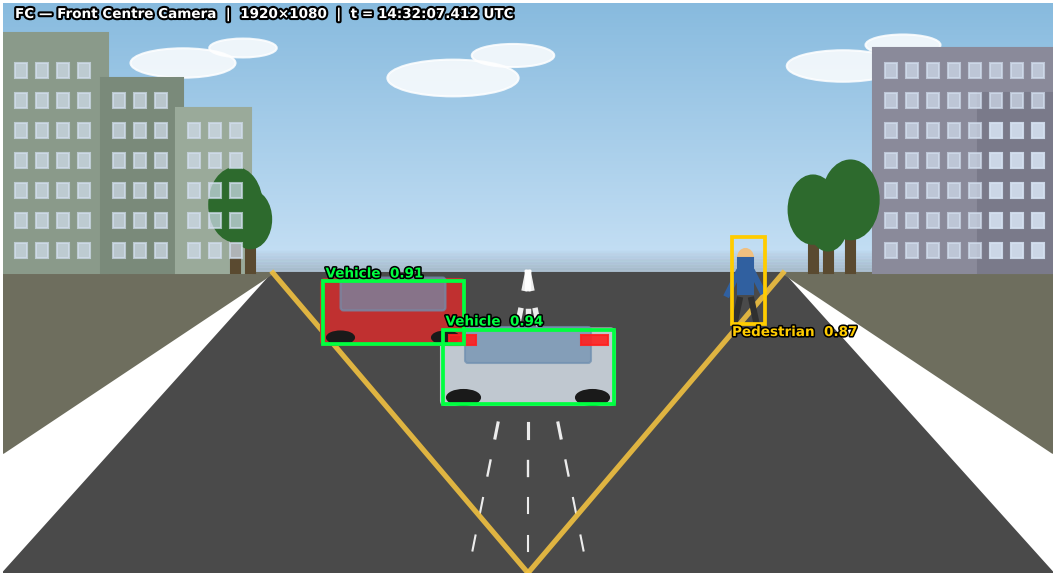
\includegraphics[width=0.92\linewidth]{figures/sample_camera.png}\\[2pt]
  \small\textbf{(a)} Front-Centre Camera frame (1920$\times$1080) with 2D bounding-box
  detections overlaid. Green boxes: vehicles; yellow box: pedestrian.
  Confidence scores from the pre-annotation object detector are shown above each box.
\end{minipage}

\vspace{8pt}

%% Row 2 — LiDAR + Radar side by side
\begin{minipage}{0.46\linewidth}
  \centering
  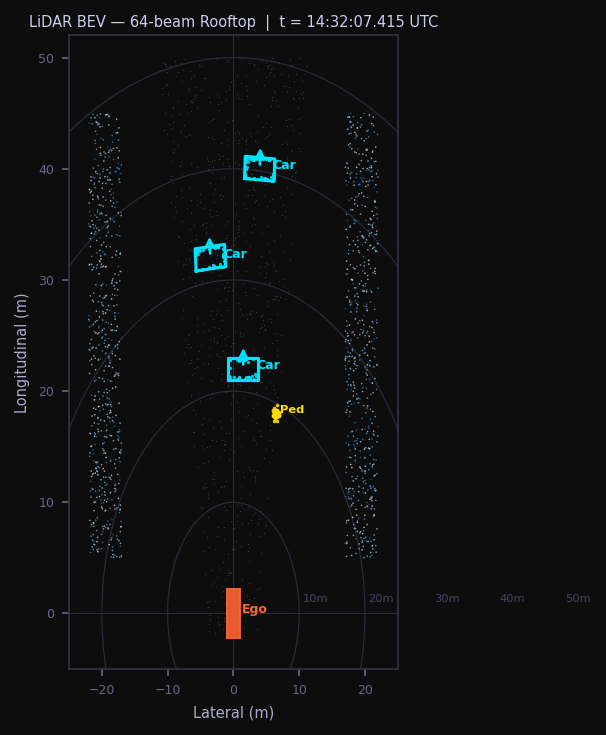
\includegraphics[width=\linewidth]{figures/sample_lidar.png}\\[2pt]
  \small\textbf{(b)} 64-beam rooftop LiDAR bird's-eye-view (BEV) point cloud.
  Cyan boxes: 3D object track projections. Yellow cluster: pedestrian.
  Orange rectangle: ego vehicle. Grey rings mark 10\,m range increments.
\end{minipage}
\hfill
\begin{minipage}{0.50\linewidth}
  \centering
  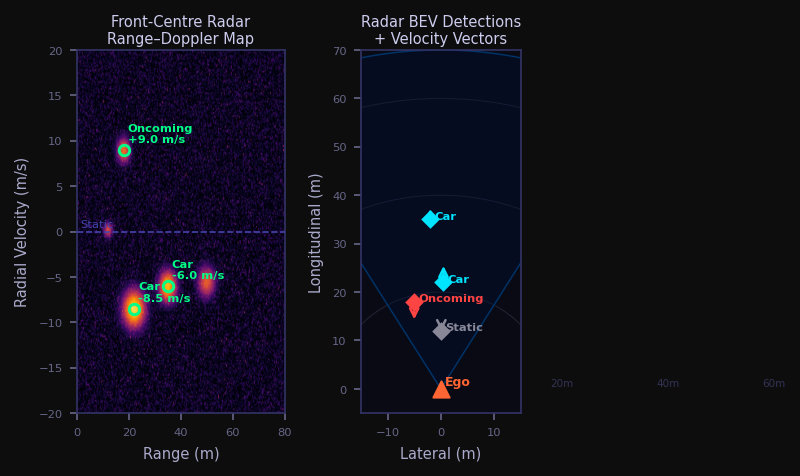
\includegraphics[width=\linewidth]{figures/sample_radar.png}\\[2pt]
  \small\textbf{(c)} Front-centre mmWave radar output. \textit{Left}: Range--Doppler
  (range--velocity) heatmap; targets circled in cyan with radial velocity labels.
  Dashed line separates approaching (negative) from receding (positive) objects.
  \textit{Right}: Radar BEV with velocity vectors (arrow length $\propto$ speed).
\end{minipage}

\vspace{4pt}
\caption{Representative sensor data samples from a single \lucid{} scenario
  (Scenario ID: SC-00842; urban intersection, daytime, clear weather).
  All three modalities are hardware-synchronised to within 1\,ms via PTP.
  \textbf{(a)} Real nuScenes surround-view camera frames from all six
  calibrated RGB cameras (1600$\times$900 each): \textit{Front Left},
  \textit{Front}, \textit{Front Right} (top row) and \textit{Back Left},
  \textit{Back}, \textit{Back Right} (bottom row), providing 360\textdegree{}
  visual coverage of the scene.
  \textbf{(b)} 64-beam LiDAR BEV point cloud with projected 3D track boxes.
  \textbf{(c)} Front-centre radar range--Doppler map and BEV detection plot
  with radial-velocity vectors.
  The simultaneous availability of all modalities at each timestep enables
  rich multi-sensor fusion research and causal annotation grounded in
  complementary sensory evidence.}
\label{fig:sensor_samples}
\end{figure*}


%% ── Figure 4: Multi-Modal Sensor Fusion BEV ─────────────────────────────────
\begin{figure}[htbp]
\centering
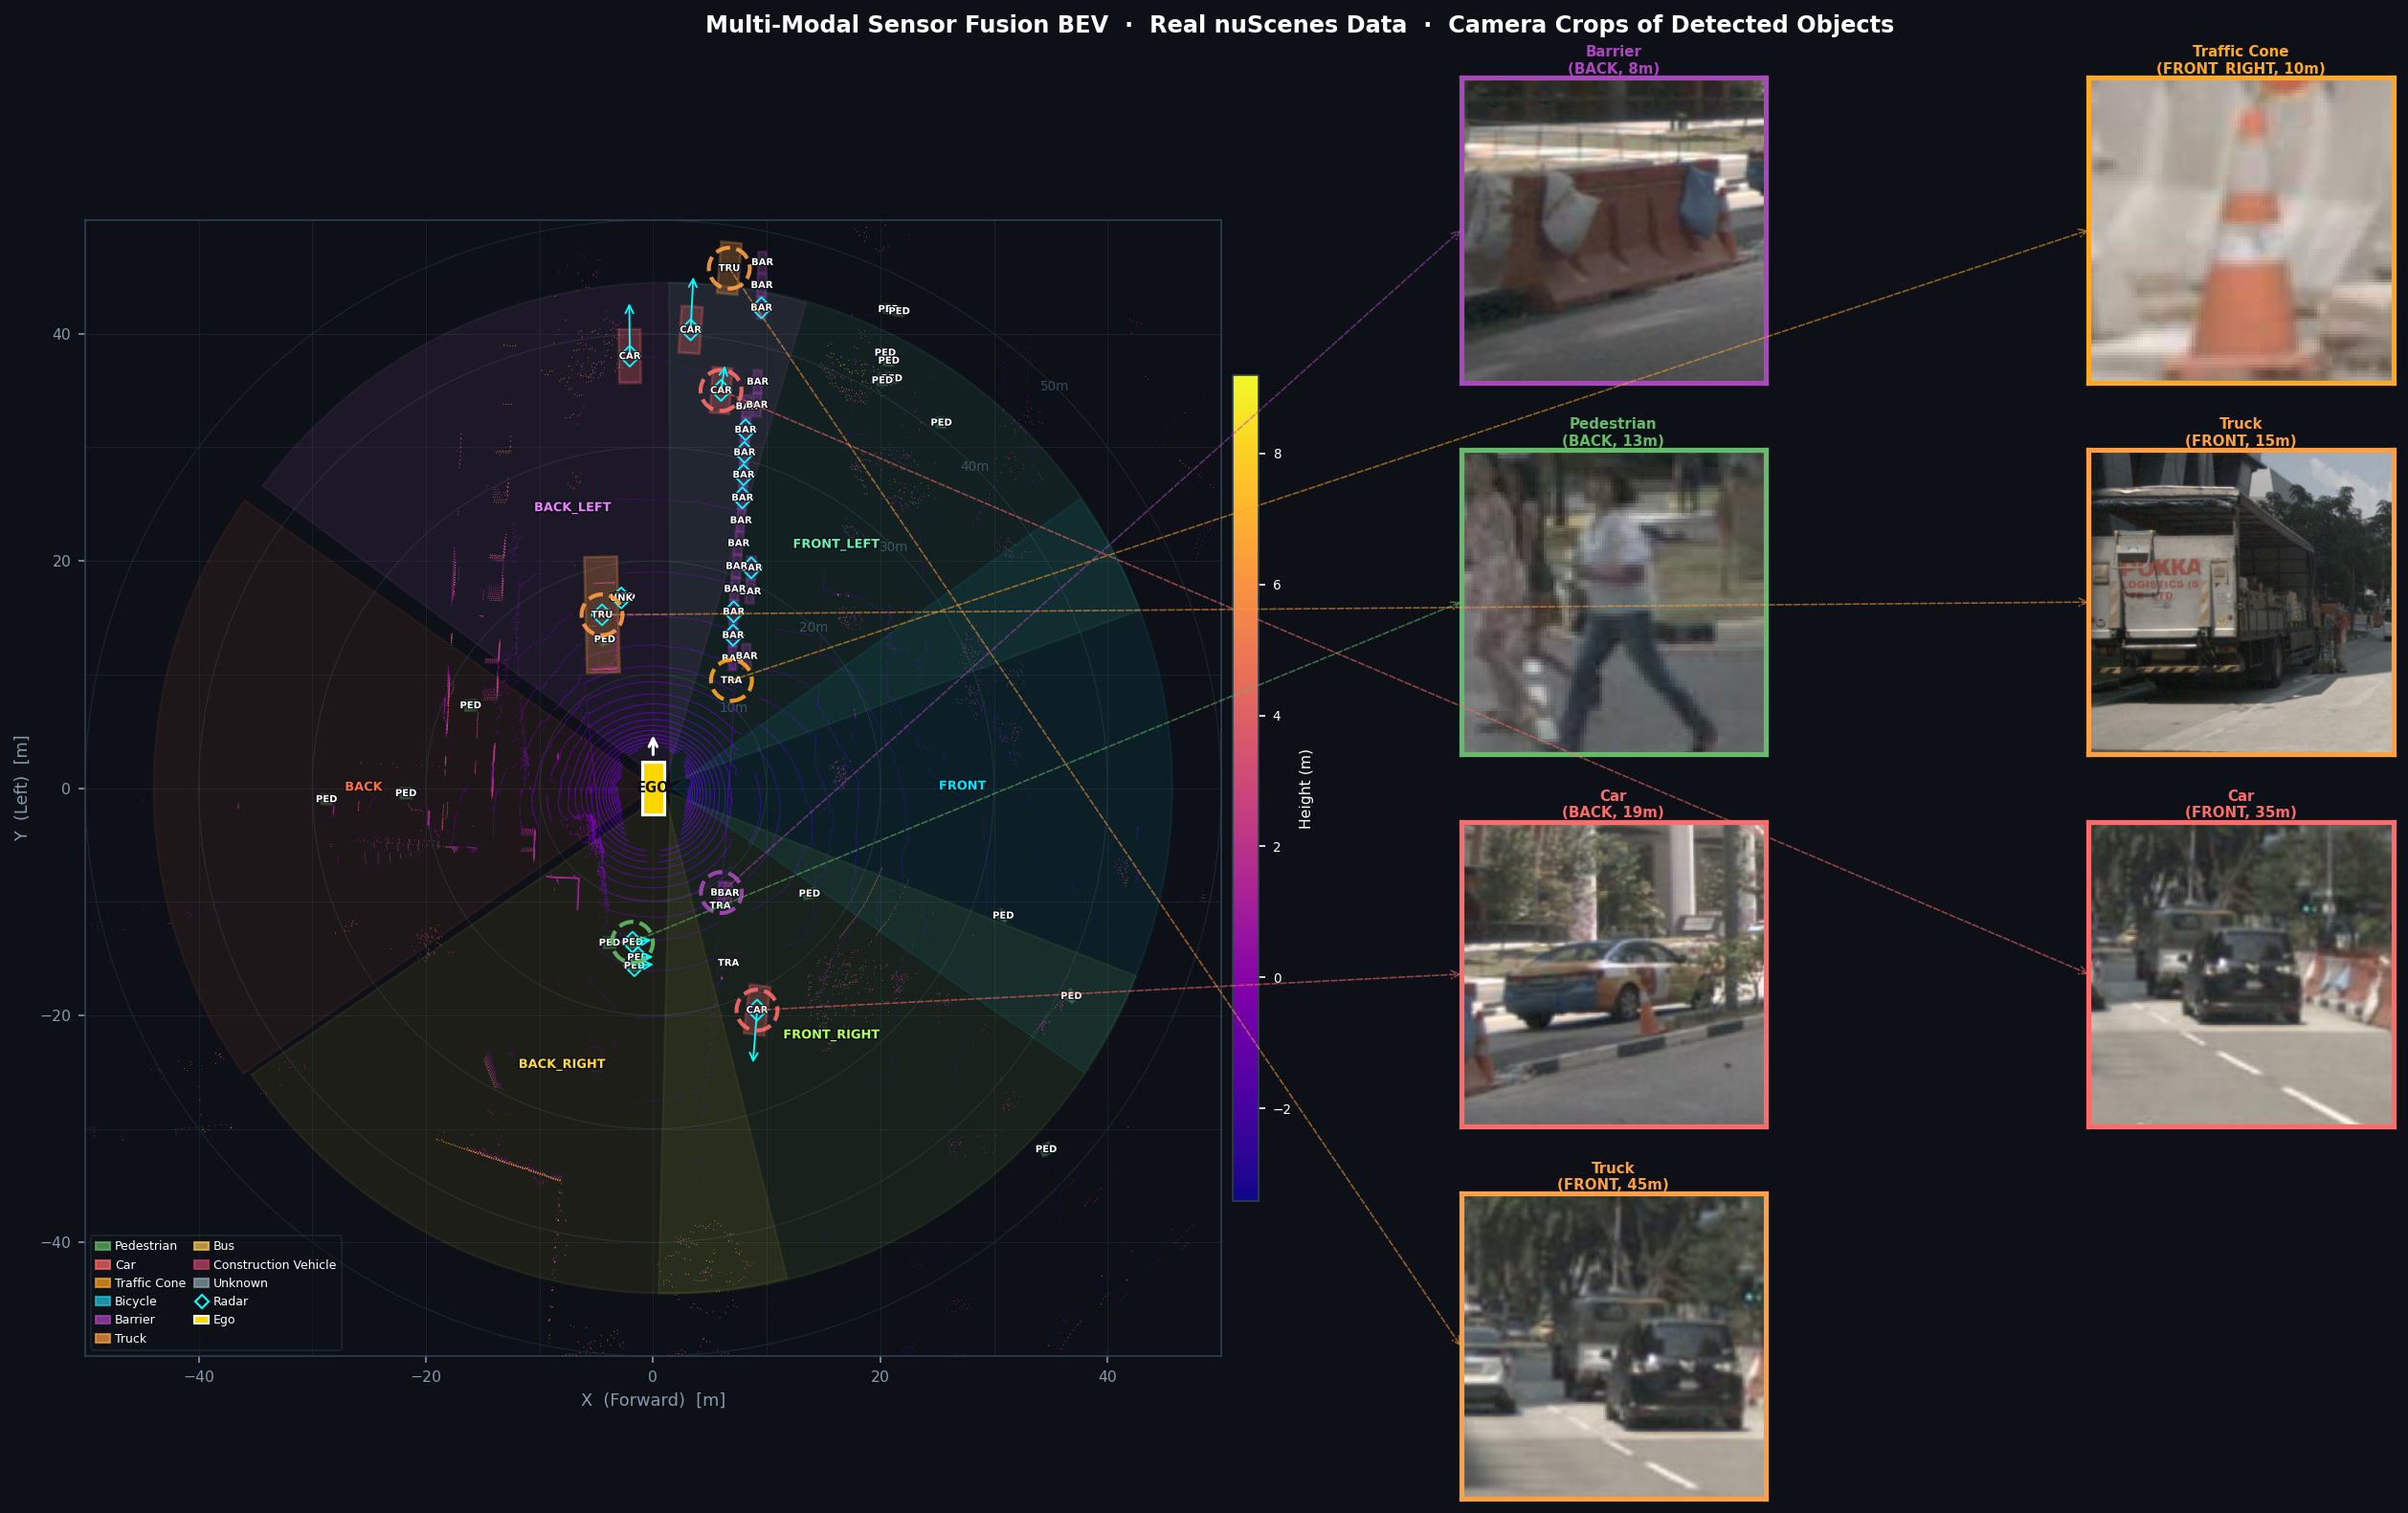
\includegraphics[width=\linewidth]{figures/sensor_fusion_bev.png}
\caption{Multi-modal sensor fusion bird's-eye-view (BEV) with real camera
  crops of detected objects, rendered from nuScenes scene
  \texttt{n015-2018-07-24-11-22-45+0800} (urban driving, Singapore).
  \textbf{Left -- BEV}: 33{,}880 height-coloured LiDAR points (plasma colourmap)
  from a Velodyne HDL-32E sweep spanning $\pm50$\,m.
  Six colour-coded wedges show camera FOV coverage; dashed rings mark
  10--50\,m range.
  Oriented bounding-box footprints (coloured by class: car, truck, pedestrian,
  barrier, traffic cone, \emph{etc.}) are projected from ground-truth 3D
  annotations; cyan diamonds with velocity arrows mark radar-confirmed
  detections.
  \textbf{Right -- Camera crops}: real image patches extracted from the
  six surround-view cameras by projecting each annotated 3D centre through
  the calibrated camera intrinsics and extrinsics.
  Dashed coloured lines link each BEV detection to its corresponding
  camera crop.
  All modalities are temporally synchronised and expressed in the
  ego-vehicle reference frame.}
\label{fig:fusion_bev}
\end{figure}
